\subsection{The Smart Home}
A “smart home” can be defined as a residence that has connected devices for various household purposes. Within the IoT industry, smart home devices represent a sub-industry of simpler, user-friendly devices that are intended to increase automation in peoples homes. These devices are intended to increase automation, and are capable of both collecting data and being controlled remotely. The areas of use may include but are not limited to: utilities such as lighting and heating, shopping, entertainment systems, and camera systems (SmartHomeUSA n.d.).

\subsection{What is Zigbee?}
Zigbee is an IEEE 802.15.4-based specification that was based around the 1990s idea of self-organizing, wireless ad-hoc networks. Wireless ad-hoc networks (WANETs) are a type of decentralized wireless architecture that relies on device-to-device communications rather than pre-existing infrastructure, such as routers or access points. 

The Zigbee Alliance was formed from a group of 25 tech-interested companies in October 2002. The group standardized the original Zigbee specification not long after in 2003, and ratified in December 2004. In 2006, the first Zigbee-based products entered the consumer market. Currently, the Zigbee Alliance members include over 400 companies and organizations from over 37 countries (“The Zigbee Alliance Celebrates 15 Years and A Decade of Standards,” 2017).

\begin{figure}[h]
	\caption{Bi-annual Shipments of Zigbee Chipsets}
	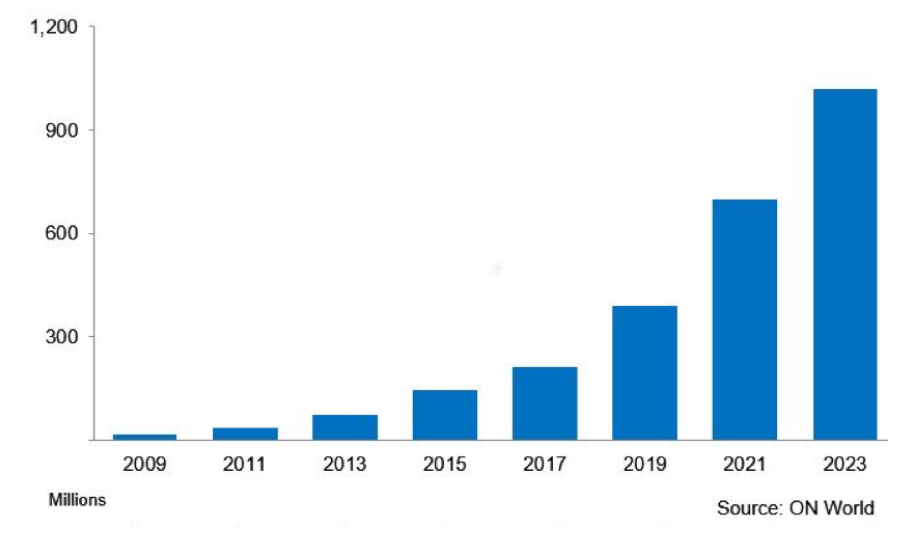
\includegraphics[width=1.0\textwidth]{sets}
\end{figure}

Zigbee chipsets are predicted to hit 1 billion shipments by 2023 (with 4.5 billion mesh devices total worldwide, most of which use Zigbee), illustrating its dominance as the most widely-used networking stack for IEEE 802.15.4 specifications. Its ease of integration with other technology stacks and hardware has seen proprietary smart home hubs such as Amazon’s Echo Plus double up as a Zigbee hub, in spite of the growth and competition from Wi-Fi and Bluetooth Low Energy (BTLE). In fact, the extremely low cost of chipsets means that developers are able to choose Zigbee/BTLE combination chips that only marginally add to the costs of manufacturing. 

Zigbee also has seen heavy adoption outside of smart home systems---commercial buildings, manufacturing and industry, municipalities, grid-based operations, and intermodal transportation systems include Zigbee as part of their technology stack (“Zigbee Leads the Wireless Mesh Sensor Network Market,” 2018). Support for medical/health devices are expected as the Zigbee Alliance looks to implement ISO/IEEE 11073 specifications into the technology stack.

The three main offerings of Zigbee are Zigbee IP, Zigbee RF4CE, and Zigbee PRO, with the lattermost being the protocol that this paper will focus on (“Network Specifications,” 2014):
\begin{itemize}
\item Zigbee IP forms the backbone of the Zigbee standard, which adds network and security layers on to the IEEE 802.15.4 standard, along with interoperability on the application layer through the Zigbee Cluster Library. It supports standard protocols such as IPv6, 6LoWPAN, TCP, TLS, UDP, and end-to-end security with TLS1.2, support for PKI, and layer 2 AES-128-CCM encryption. 
\item Zigbee RF4CE, or Radio Frequency for Consumer Electronics, offers a simple two-way, device-to-device control communication that does not require the full-featured mesh networking capabilities of Zigbee IP. 
\item Zigbee PRO is a more fully-fleshed out specification for full mesh networking capable of supporting hundreds to thousands of devices on a single network, including self-powered/energy-harvesting devices. Most developers colloquially consider non-PRO Zigbee to be a legacy, with Zigbee PRO being the standard moving forward.
\end{itemize}

\subsection{The Zigbee PRO Protocol}

The application layer gives the developer easy to use access to the data communicated over the network layer below. While the application itself is the element that will vary the most between different IoT devices, the communication needs of devices that report data and are fairly similar and limited to sending and receiving commands and data. The lack of homogeneity is instead driven by the unique physical constraints on IoT devices. Some devices, like a refrigerator that can send you a live feed of its contents, are plugged into the wall and do not need to limit their power consumption. Others, like a small sensor that checks whether a door is closed, must conserve limited battery resources as carefully as possible to avoid irritating the owner of the device. The application layer must be configured differently for each of these cases.

The network layer bridges the divide between the application layer and the physical signals received and transmitted by the radio. It also includes software used to route that data to different locations by different methods: the specification allows for a hub-and-spoke model (peripheral sensors report their data to a single devices that sends back commands), a mesh network (any device can talk to any other device), and a tree network (nodes can be simultaneously a hub to some devices and a peripheral to others). A hub-and-spoke model is the most straightforward to implement and the hub would most likely go on to report data to the internet at large to report to the company that created the devices. A mesh network is very resilient since no one point is the weakest, unlike the other two models where the hub or root of the tree are essential to operation. A tree model is good for enforcing a nuanced hierarchy of different devices, which might reflect the tasks devices are responsible for, the level of injury that a device can inflict, or the distance data can travel.

\begin{figure}[h]
	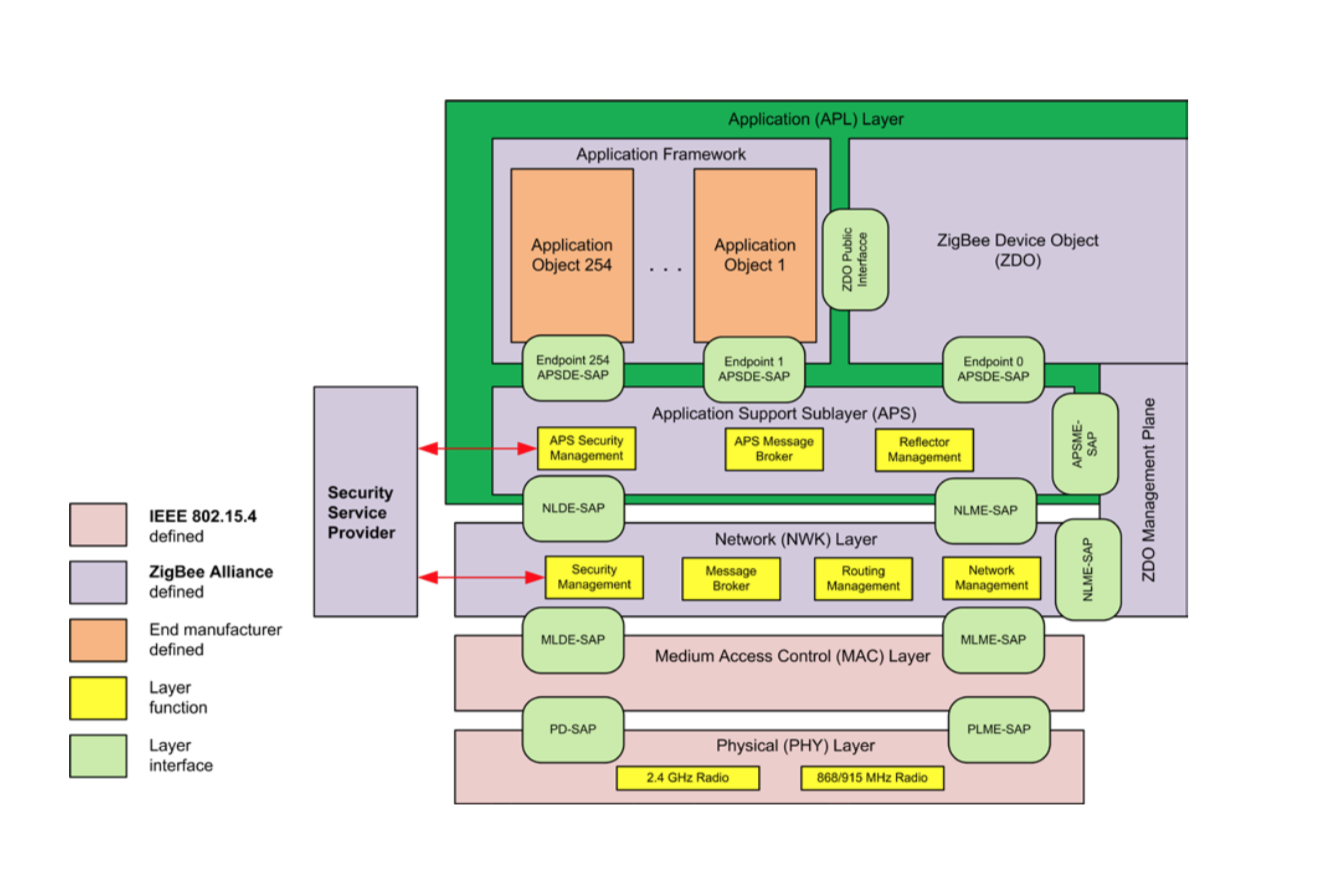
\includegraphics[width=1.0\textwidth]{top}
\end{figure}

\subsection{Threat Model: Adversaries}
Different attackers have wildly different capabilities, and therefore a suitable defense against one may be wildly insufficient (or overkill) against another. In This World Of Ours, James Mickens breaks attackers down into two basic categories: those representing governments and militaries, with effectively unlimited resources, and everyone else. (Mickens, 2014) In the case of home automation for the average, non-nation-state-actor consumer, it is reasonable to assume with some caveats that any attacker will have limited resources and all possible attacks will not be realistic. 

Mickens briefly identifies a third category of attacker: the metaphorical (or perhaps literal) angry ex-girlfriend/boyfriend, representing someone who knows the user well, may have some but not excessive technical adeptness and resources, and may have physical access. While it is important not to overlook the potential role of home automation in domestic abuse and similar situations of interpersonal violence, a New York Times report notes that the problem is usually a combination of one party having installed devices, and therefore having administrative control of them, and restraining orders and other legal measures not taking this potential means of abuse into account (Bowles). Because direct regulation of IoT is unlikely to be the best solution to this problem, this type of attack will be considered beyond the scope of this paper.

This leaves the category of attackers who are neither politically nor personally motivated. Such attackers are generally motivated by some combination of money and notoriety, and may monetize access to a stranger’s IoT device in many ways, including the following (DeSombre, 2018):
\begin{itemize}
\item Financial fraud: The attacker may directly harvest credentials and/or financial details, or they may learn other personal information which can then be used in a spearphishing attack.
\item Cryptojacking: The attacker may run cryptomining software on the victim’s device, essentially stealing computing power and electricity from them.
\item Ransomware: The attacker may implant malware than encrypts information and extorts the victim for it.
\item Botnet recruitment: The attacker may use the device to spread malware, send spam emails, participate in DDoS attacks, and so on. Aside from stolen computational resources, no money is directly taken from the victim in this case; hackers may instead charge others for the botnet’s services.
\end{itemize}

\subsection{Zigbee-Specific Vulnerability Analysis}
This section briefly evaluates how the concepts discussed in the threat model relate specifically to the Zigbee protocol. Zigbee is particularly vulnerable to attacks in which the attacker is physically near the device, and older versions add new devices in a way that is insecure. Correct implementation is key to maintaining security.

\subsection{Data Security}
Zigbee encrypts data using AES-128, a very well-established algorithm. The correctness of the algorithm itself can be considered out of scope---if AES-128 is shown to be breakable, such an exploit applied to home automation devices would be the least of everyone’s problems. The aspects of data encryption that are up to Zigbee developers are (i) correct implementation, and (ii) actually encrypting everything that should be encrypted.

Zigbee 1.2 has a known period of insecurity while a new device is being added, with developers noting it as a security vs. simplicity tradeoff and arguing that it is not feasible to have consumers instead enter security codes on all devices, since some IoT devices such as light bulbs have no reasonable means of direct user I/O (Hardawar 2015). They point out that if setting up encryption is too complicated, the user will simply not do it at all, which is far worse than accepting a split-second period of vulnerability while a secret key is being broadcast in cleartext.

Tools exist to sniff traffic and capture the unencrypted key, although exploitation requires the attacker being on the network---requiring physical proximity---during the time the key is being exchanged. Such an exploit was demonstrated at the 2015 BlackHat conference (Zillner, 2015). Zigbee 3.0 patches this flaw (Zigbee: Securing the Wireless IoT, 2017).

Because Zigbee only offers an interface to the application layer, it does not play a role in determining what data is sent to the manufacturer, and so the issue of user data being sent to manufacturers against the user’s wishes is not a part of Zigbee’s threat model.

\subsection{Device Security}
As part of the network stack, Zigbee libraries are likely to process significant amounts of untrusted, outside-originating, and therefore possibly attacker-controlled data. A bug in the Zigbee implementation---that is, something like a buffer overflow or use-after-free\footnote{These are specific, common programming errors that allow an attacker to force a machine to execute the attacker’s code rather than the intended code. They happen at a lower level of abstraction than errors such as incorrect protocol implementation that cause sensitive information not to be encrypted. In large code bases, it is very difficult to ensure that no such errors are present, and tools for definitively proving their absence are difficult to apply and have not yet found their way into widespread industry use.
} allowing for control flow hijacking, not necessarily an error in the protocol itself---would allow an attacker to take over the device.

Several attacks against device security have been demonstrated. The Python library Killerbee offers a utility for crashing Zigbee devices by connecting many spoofed stations. In itself, this is a sort of DOS attack; it also has applications as a phase of a more complete compromise, since crashed devices must reconnect to the network upon rebooting and, depending on manufacturer implementation, may broadcast keys insecurely.

In another case, researchers exploited the Zigbee stack in Philips Hue Light Bulbs to spread a worm to other devices (Ronen, 2018). They were able to remotely control lights. In addition to the obvious safety hazards and the previously-discussed possibility of devices being used in botnets, cryptomining, etc., malware spread to proximal devices presents a threat to the power grid - by controlling many devices that are located close to one another, an attacker can sharply vary the draw on a portion of the grid, which may temporarily impact availability or even damage equipment.

\subsection{Policy Landscape}
Privacy breaches are mostly covered under various privacy laws in the US, and under “data protection” rules in the European Union. In both regions, the legal frameworks draw on fair information practice principles (FIPPs) that include Transparency, Individual Participation, Purpose Specification, Data Minimization, Use Limitation, Data Quality and Integrity, Security, Accountability, and Auditing (DHS, 2014). However, different agencies emphasize different subsets of these principles. For example, while the EU legislation GDPR covers all data controllers across all industries, privacy laws are mostly domain specific in the U.S. Moreover, while there is common ground in goals on how to address privacy harms, such as advocating privacy by design, enhanced data security, and access rights to check and correct data, there are differences in how to implement these goals (in terms of obtaining consent, notification of data breaches, cross-border data flows).

\subsection{Established Regulatory Concepts}
\subsubsection{Right to be Forgotten}
Right to be forgotten provides the right to the consumer to ask for erasure of all their personal data unless there is a legitimate reason for the company to keep it (i-scoop, n.d.-b). Europe has led the efforts in identifying right to be forgotten as a fundamental right which is now accepted in other major privacy rules and regulations as such (Spiegel, 2014). 

The way this right is handled in GDPR is a good example of how the policy does not specify the technical requirements to be implemented by service providers, but simply defines the right and puts the liability on data aggregators in case of a violation. In the Home IoT context, this approach can create some ambiguity for service providers as they identify and implement new methods for how they structure data, the retention periods for different types of data, etc. (zeb, 2017).

\subsubsection{Vulnerability Notification}
The push for service providers to disclose any vulnerabilities so that the public is aware and can take necessary measures to protect themselves from further damage is another policy item that is widely accepted by most stakeholders. This principle is included in some of the policy documents shown in the table above. The industry leaders are also supporting this principle; for example, disclosure requirements were recently highlighted as a key action item by Google’s Framework for Responsible Data Protection Regulation (Enright, 2018). Transparency requirement can be seen as an alternative solution to the fact that no tamper-proof technology is available and transparency is the first step for the IoT community to do a better job in identifying problems and addressing them effectively. 

\subsubsection{Data Portability}
Defined as a fundamental right of the consumer in GDPR, data portability is a new concept (i-scoop, n.d.-a). The right to data portability is consumer centric regulation that aims to foster competition among service providers with the goal that the consumer will be able to switch between services with minimal replacement costs. GDPR defines two types of data under the portability requirement: personal data and observed data, which is the data a service provider collects as observation data while the consumer uses the service. The second data category includes IoT data. Again, data portability is required as a consumer right in the instances we observed, leaving room for service providers to identify best ways to comply as long as they take on the liability to fulfill the consumers’ needs.
